\section{Productivity Focused Platforms} \label{chapter3:software-productivity}

\cit{It is becoming increasingly important to the data-proces\-sing industry to be able to produce
[programming systems] % more programming systems and produce them with fewer errors,
at a faster rate, and in a way that modifications can be accomplished easily and quickly.}{W. Stevens, G. Myers, L. Constantine \cite{Stevens1974}.}

In order to improve and maintain a software system, it is important to holds in mind a mental representation of its implementation \cite{Simon1962}.
As the system grows in size, the mental representation becomes more and more difficult to grasp.
Therefore, it is crucial to decompose the system into smaller subsystem easier to grasp individually.

% \cit{Measuring programming progress by lines of code is like measuring aircraft building progress by weight.}{Bill Gates}

Section \ref{chapter3:software-productivity:modularity} presents the modular programming paradigms, and their programming models, oriented toward productivity.
Section \ref{chapter3:software-productivity:adoption} presents the adoption of the implementations of modular programming languages.
Section \ref{chapter3:software-productivity:efficiency-limitations} presents the consequences of the modularity on performance.
Finally, section \ref{chapter3:software-productivity:summary} summarizes the three previous sections in a table.

\subsection{Modular Programming} \label{chapter3:software-productivity:modularity}

\begin{figure}[!h]
\begin{center}
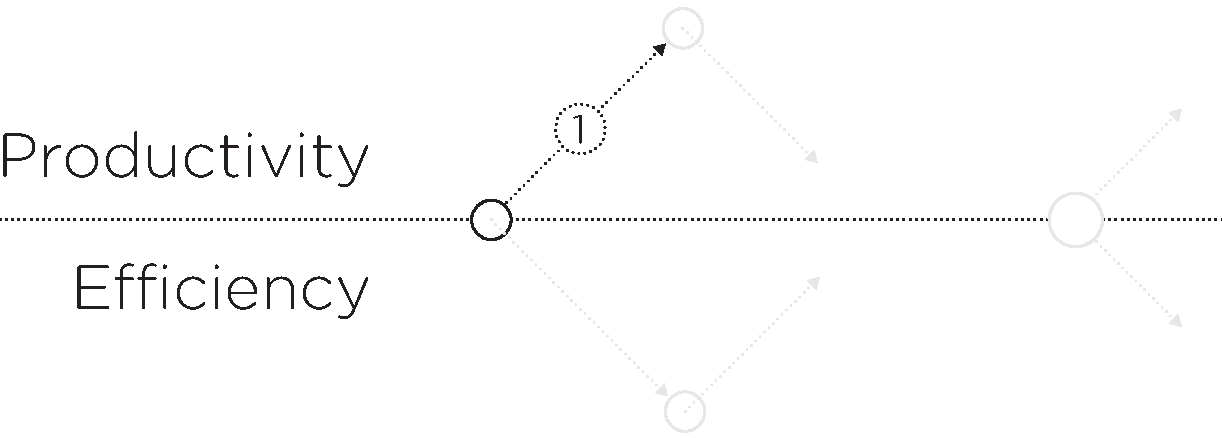
\includegraphics[width=0.6\textwidth]{../resources/state-of-the-art-1.pdf}
\end{center}
\caption{Focus on Productivity}
\label{fig:state-of-the-art-1}
\end{figure}

The next paragraphs presents the different programming model regarding their support to modular programming and productivity.

\subsubsection{Imperative Programming}

\illustration{spaghetti programming}
\illustration{lasagna programming}

Imperative programming is the very first programming paradigm, as it evolves directly from the hardware architectures.
It allows to express the suite of operation to carry sequentially on the computing processor.
Most imperative languages provide encapsulation with modules but not higher-order programming. % , nor lazy evaluation.
The implementations of Imperative Programming are \ImplementationsOf{Imperative Programming}.

\subsubsection{Object Oriented Programming}

\illustration{multiple cells communicating}

The very first Object-Oriented Programming (OOP) language was Smalltalk \cite{Goldberg1984}.
It defined the core concepts as message passing and encapsulation %, and dynamic binding
\ftnt{http://userpage.fu-berlin.de/~ram/pub/pub\_jf47ht81Ht/doc\_kay\_oop\_en}.
Nowadays, the emblematic figures in the software industry are \ImplementationsOf{Object-Oriented Programming}.
They provide encapsulation with Classes, and allows mutable structures for performance reasons.
They recently introduced higher-order programming with lambda expressions.

\subsubsection{Functional Programming} \label{chapter3:software-productivity:programming-models:functional-programming}

% \cit{All problems in computer science can be solved by another level of indirection}{Butler Lampson}

The definition of pure Functional Programming resides in manipulating only expressions and replacing state mutability, with immutable message-passing.
The absence of state mutability makes a function side-effect free, hence their execution can be scheduled in parallel.
The most important pure Functional Programming languages are \ImplementationsOf{Functional Programming}.
They provide encapsulation, higher-order programming and lazy evaluation.

\subsubsection{Multi-Paradigm}

The functional programming concepts are also implemented in other languages along with mutable states and object-oriented concepts.
Major recent programming languages, including Java 8 and C++ 11, now commonly present higher-order functions.
\textit{In fine}, it helps developers to write applications that are more maintainable, and favorable to evolution \cite{Hughes1989,Turner1981}.
These recent multi-paradigms languages such as \ImplementationsOf{Multi Paradigm} combine the different paradigms to help developer building applications faster.

\separator

The previously presented programming models are all rather focused on productivity, as recapped in table \ref{tab:productivity-modularity}.

\ModularProductivityTable{tab:productivity-modularity}

\subsection{Adoption} \label{chapter3:software-productivity:adoption}

As stated previously, adoption relies an productivity as well as efficiency.
The next paragraphs present the adoptions of different platforms for web development and focus on Javascript.

\begin{figure}[!h]
\begin{center}
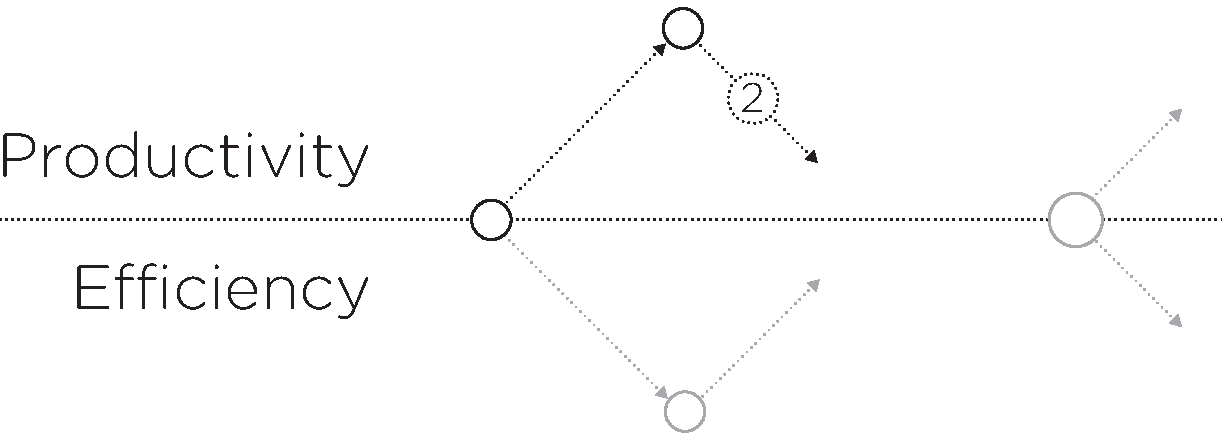
\includegraphics[width=0.6\textwidth]{../resources/state-of-the-art-2.pdf}
\end{center}
\caption{Steering back toward Performance Efficiency}
\label{fig:state-of-the-art-2}
\end{figure}

\subsubsection{Community}

\paragraph{Available Resources}

As of December 2015, Javascript ranks 8th according to the TIOBE Programming Community index, and was the most rising language in 2014.
This index measure the popularity of a programming language with the number of results on many search engines.
And it ranks 7th on the PYPL.
The PYPL index is based on Google trends to measure the number of requests on a programming language.

From these indexes, the major programming languages are Java, C++, C, C\# and Python.
These languages are still widely used by their communities and in the industry.

\begin{figure}[h!]
  \centering
  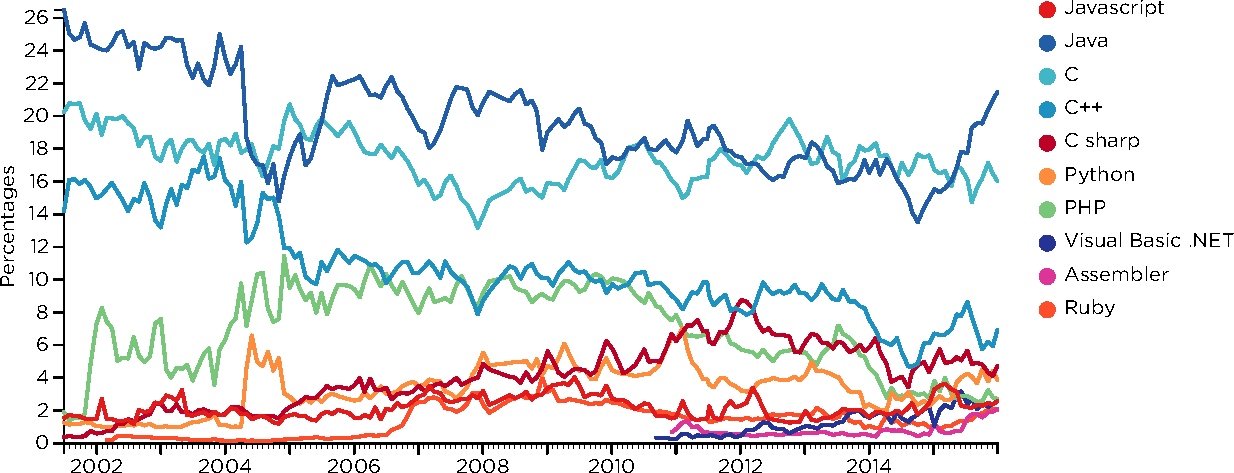
\includegraphics[width=\linewidth]{../resources/tiobe.pdf}
  \label{fig:tiobe}
  \caption{TIOBE ranking}
\end{figure}

\paragraph{Developers Collaboration Platforms}

Online collaboration tools give an indicator of the number of developers and projects using certain languages.
Javascript is the most used language on \textit{Github}\ftnt{the most important collaborative development platform gathering about 9 millions users.} and the most cited language on \textit{StackOverflow}\ftnt{the most important Q\&A platform for developers.}.
It represents more than \num{320000} repositories on \textit{Github}.
The second language is Java with more than \num{220000} repositories.
It is cited in more than \num{960000} questions on \textit{StackOverflow} while the second is Java with around \num{940000} questions.
And according to a survey by \textit{StackOverflow}, it is currently the language the most popular\ftnt{http://stackoverflow.com/research/developer-survey-2015}.
Moreover, the Javascript package manager, \textit{npm}, has the most important and impressive package repository growth.

% \begin{figure}[h!]
%   \centering
%   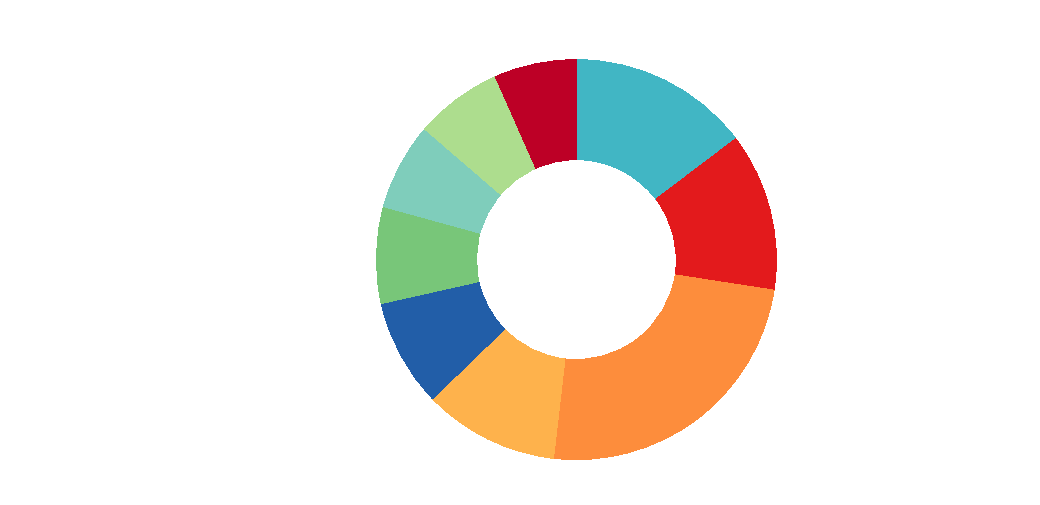
\includegraphics[width=0.7\linewidth]{../resources/stackoverflow-mostwanted.pdf}
%   \label{fig:so-tags}
%   \caption{Most Wanted Technologies in 2015 from a StackOverflow survey}
% \end{figure}

\begin{figure}[h!]
  \centering
  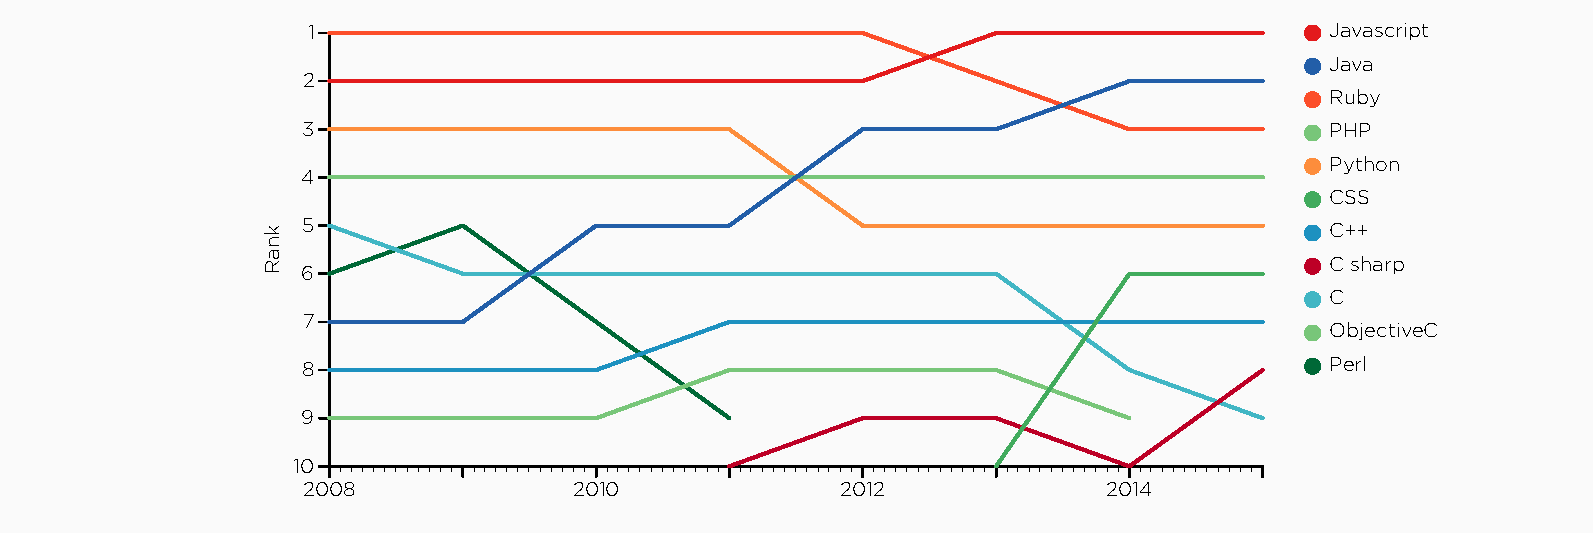
\includegraphics[width=\linewidth]{../resources/github-languages.pdf}
  \label{fig:github-languages}
  \caption{Languages Ranks from number of Github projects}
\end{figure}

\begin{figure}[h!]
  \centering
  
\includegraphics[width=\linewidth]{../resources/stackoverflow-tags.pdf}
  \label{fig:so-tags}
  \caption{StackOverflow Tags evolution}
\end{figure}

\begin{figure}[h!]
  \centering
  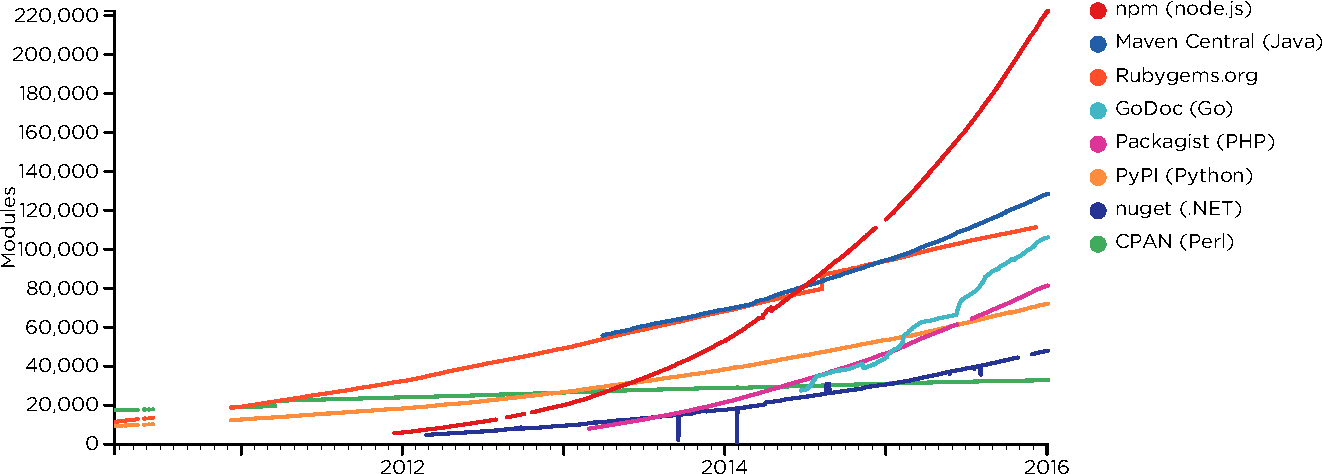
\includegraphics[width=\linewidth]{../resources/modulecounts.pdf}
  \label{fig:modulecounts}
  \caption{Module Counts per package manager}    
\end{figure}

\subsubsection{Industry}

The industrial actors avoid to discolse their activities beliving it grants them an edge on the competition.
The previous metrics represent the visible activity but are barely representative of the software industry.
The trends on job opportunities give some additional hints on the situation.
Javascript is the third most wanted skill, according to \textit{Indeed}\ftnt{http://www.indeed.com}, right after SQL and Java.\ftnt{http://www.indeed.com/jobtrends?q=Javascript\%2C+SQL\%2C+Java\%2C+C\%2B\%2B\%2C+C\%2FC\%2B\%2B\%2C+C\%23\%2C+Python\%2C+PHP\%2C+Ruby\&l=}
Moreover, according to \textit{breaz.io}\footnote{\textit{breaz.io} \url{https://breaz.io/} was recently acquired by \textit{hired} \url{https://hired.com/}.}, Javascript developers get more opportunities than any other developers.
Javascript is increasingly adopted in the software industry.

\separator

According to these various sources, multi paradigm languages like Javascript are the most widely used by the community and the industry, as presented in table \ref{tab:productivity-adoption}.
OOP and Imperative Programming remains strong in the industry, but are progressively abandoned by the community.
Functional Programming is not well represented in community nor the industry.

% Table \ref{tab:productivity-adoption} presents a summary of the analysis of the programming models presented in the previous paragraphs.

\ModularAdoptionTable{tab:productivity-adoption}

\subsection{Efficiency Limitations} \label{chapter3:software-productivity:efficiency-limitations}

Eventually, the presented languages are hitting a wall on their way to performance.
They provide global memory abstraction on which to rely to assure encapsulation and composition. % -- either mutable state or immutable state.
Functional programming relies on immutable message-passing.
It might impact performance at a fine-grain level because of heavy memory usage.
And the synchronization required by mutable state is often hard to develop with \cite{Adya2002}, or avoid parallelism \cite{Pai1999,Krohn2007}.
These results are recapped in table \ref{tab:productivity-performance}.

\ModularEfficiencyTable{tab:productivity-performance}

The only solution to provide performance efficiency is to combine mutable state at a fine-grain level and immutable state at a coarse-grain level \ftnt{http://joeduffyblog.com/2010/07/11/thoughts-on-immutability-and-concurrency/}.
That is to provide both synchronization and message-passing to allow parallelism.
The platforms extending these languages with concurrent or parallel paradigms to improve efficiency are addressed in the next section.

\subsection{Summary} \label{chapter3:software-productivity:summary}

The evaluation of the platforms presented in this section is summarized in table \ref{tab:productivity-synthesis}.

\ModularSummaryTable{tab:productivity-synthesis}















\endinput

Octave and python: higher-level scripting languages productivity and performance evaluation, by Chaves, Nehrbass, Guilfoos, Gardiner.
Haskell vs Ada vs C++ vs Awk vs ... an experiment in software productivity, technical report by Hudak and Jones.
An empirical comparison of seven programming languages, by Prechelt.


remote first Zack Holman : promote asynchronous communication
\ftnt{http://zachholman.com/posts/remote-first/}
+
Conway's law
\cit{Organizations which design systems [...] are constrained to produce designs which are copies of the communication structures of these organizations.}
{M. Conway \cite{Conway1968}}


What makes a great software engineer? \cite{Li2015}

About great software development:
Productivity : Sackman et. al 68, Gugerty & Olson 86
Collaboration, meaningful contribution : Kelly 99, Begel & Simon 06, Hewner & Guzdial 10
Communicate and acquire understanding : LaToza 06, Ko 06
Technical Knowledge : 
Open minded : McConnell 04, Bryant 13


Compiler productivity language into perfomance language
\cite{Kuper2015}\nt{TODO update biblio entry}